\section{Liquid Crystal-based RISs}

In this section, we first present the basic operating principles of \gls{NLC} technologies. Subsequently, we introduce two of the existing \gls{NLC}-\gls{RIS} implementations, as well as the hardware components required for implementing them.

\subsection{Basic physical principles of LC technology}\label{Sec:Basic}

\textbf{Phase shifting capability:}  
The working principle of \gls{NLC} is based on its electromagnetic anisotropy\footnote{\gls{NLC} molecules exhibit different electromagnetic properties depending on their relative orientation with the \gls{RF} electric field.}. In particular, due to the ellipsoidal shape of \gls{NLC} molecules, the \gls{NLC} presents a larger permittivity (i.e., higher phase shift) when the electric field, $\vec{E}_{\rm RF}$, is aligned with the major axis of the molecules, $\vec{n}$, than when it is aligned with  the minor axis (i.e., lower phase shift), see~Fig.~\ref{fig:LCmolres}. Therefore, by controlling the orientation of \gls{NLC} molecules, we can alter the phase shift of the \gls{RF} signals. 

 % \subfloat[]{
 %        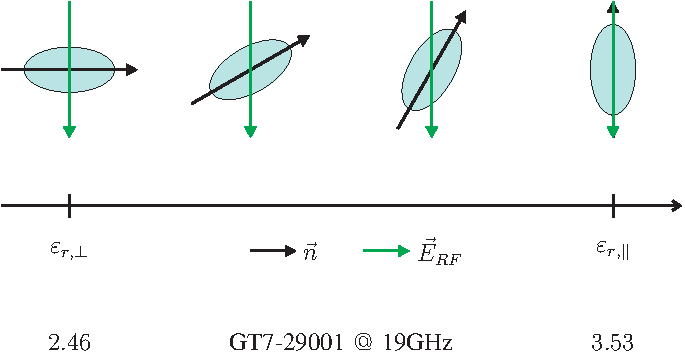
\includegraphics[width=0.7\columnwidth]{Figures/LCmolecules.pdf}
 %        \label{fig:LCmoledulces}
 %    }\hfill
	% \subfloat[]{
	% 	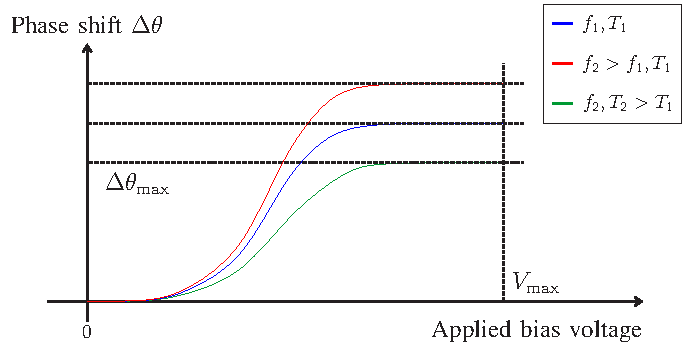
\includegraphics[width=0.8\columnwidth]{Figures/LCresponse.pdf}
	% 	\label{fig:LCresponse}
 %    }
    


%To exploit the above feature of \glspl{NLC}, the orientation of the LC molecules should be changed in a controlled manner.  

This is achieved by placing a thin \gls{NLC}-layer between two electrodes. Thereby, when no voltage is applied, the molecules are in their relaxed phase, where $\vec{E}_{\rm RF}$ is perpendicular to $\vec{n}$, and hence \gls{NLC} shows a minimum permittivity $\varepsilon_{r,\perp}$. In contrast, when the maximum voltage is applied, the \gls{NLC} molecules orient along the induced external electric field, which leads to $\vec{E}_{\rm RF}$ being now parallel to $\vec{n}$ and hence a maximum permittivity of $\varepsilon_{r,\parallel}$. The maximum achievable phase shift, $\Delta\theta_{\max}$, therefore scales with $\Delta\varepsilon = {\varepsilon_{r, \parallel}} - {\varepsilon_{r, \perp}}$.  The \gls{NLC}-layer permittivity and the corresponding maximum achievable phase-shift are dependent on the operating frequency as well as temperature, cf. Fig.~\ref{fig:LCmolres}, which will be elaborated further in Section~\ref{sc:challenges}. 

\textbf{Response time:} The alignment of the \gls{NLC} along the electrodes when applying a voltage (for positive phase shifts) is faster than the alignment of the molecules due to mechanical anchoring forces (for negative phase shifts). For this reason, usually the latter slow transition is considered and modelled by the decay or switch-off response time, $\tau_{\rm off}$, which is proportional to $\tau_{\rm off} \propto {\gamma_{\rm rot}{d_{\rm LC}^2}}/{K_{11}}$,  where  $\gamma_{\rm rot}$ is the rotational viscosity, $d_{\rm LC}$ is the \gls{NLC}-layer thickness, and $K_{11}$ is the splay deformation factor of the \gls{NLC}. Therefore, the response time can be reduced by adopting a narrower \gls{NLC} layer; however, this implies more delicate (hence costly) manufacturing and higher conductor losses, motivating research to reduce losses in thin phase shifters \cite{neuder2023compact}.  The \gls{NLC} thickness, $d_{\rm LC}$, can be as low as a few \SI{}{\micro\meter} for switch-off response times, $\tau_\mathrm{\rm off}$, in the order of tens of milliseconds. 

\begin{figure}[t]
	\centering
 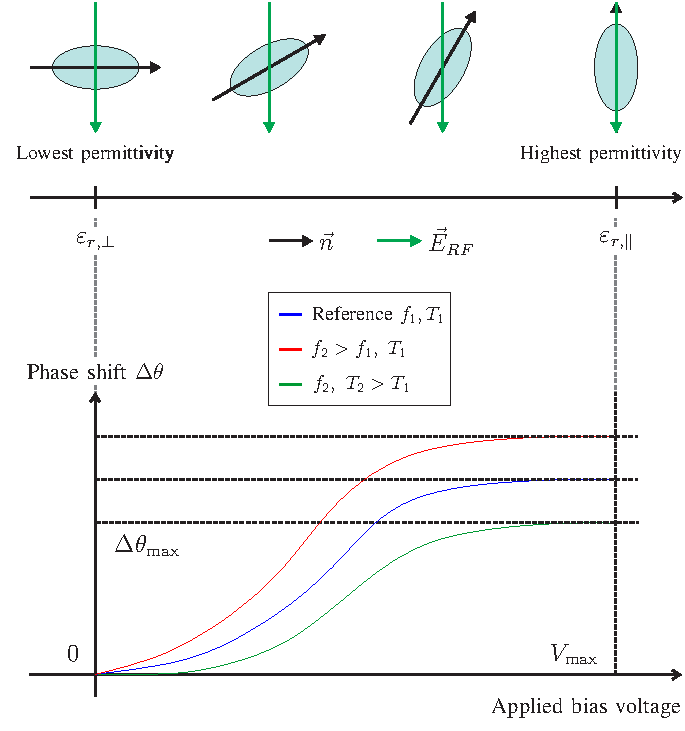
\includegraphics[width=0.8\columnwidth]{Figures/LCmolres.pdf}
	\caption{Top figure: Observed \gls{NLC} permittivity depending on the orientation between the \gls{RF} electric field, $\vec{E}_{RF}$, and the \gls{NLC} molecule major axis, $\vec{n}$. The lowest permittivity, $\varepsilon_{r,\perp}$, is observed when $\vec{E}_{RF}$ and $\vec{n}$ are orthogonal while the highest permittivity, $\varepsilon_{r,\parallel}$, is observed when $\vec{E}_{RF}$ and $\vec{n}$ are parallel to each other. Bottom figure: Schematic illustration of the corresponding phase shift achieved by applying bias voltage leading to the change in permittivities. This figure illustrates that the achievable phase shift depends on the operating frequency $f$ and temperature $T$.}
 		\label{fig:LCmolres}
\end{figure}

% \begin{figure*}[t]
% 	\centering
% \subfloat[]{
%         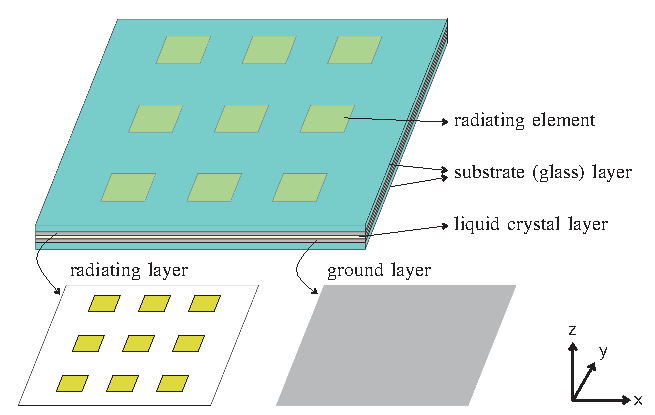
\includegraphics[width=0.8\columnwidth]{Figures/LCrisRA.pdf}
%         \label{fig:LCrisRA}
%     }\hskip 1cm
%     \subfloat[]{
%         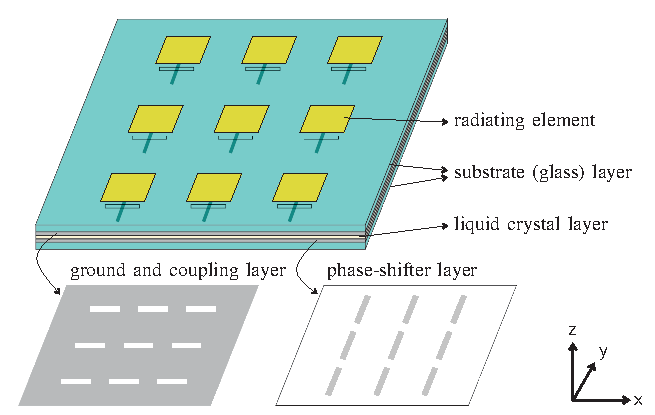
\includegraphics[width=0.8\columnwidth]{Figures/LCrisPA.pdf}
%         \label{fig:LCrisPA}
%     }\hfill
% 	\subfloat[]{
% 		\includegraphics[width=0.95\columnwidth]
%   {Figures/LCunitRA.pdf}
% 		\label{fig:LCunitRA}
%     } \hskip 0.1cm
%     \subfloat[]{
% 		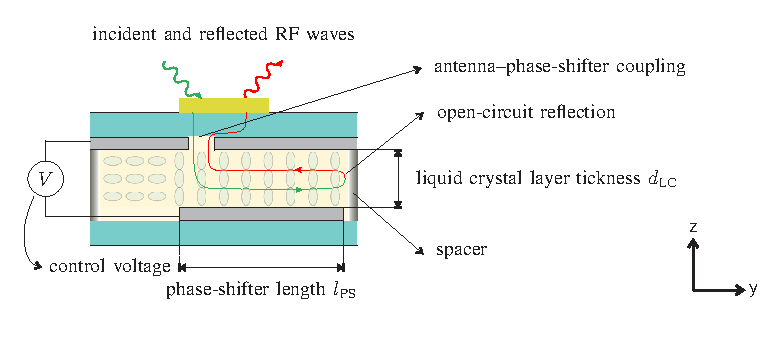
\includegraphics[width=0.95\columnwidth]{Figures/LCunitPA.pdf}
% 		\label{fig:LCunitPA}
%     } 
%     \caption{Schematic illustration of reflect-array (left-hand side) vs. phased-array (right-hand side) LC-based RISs. The top figures illustrate the implementation of LC-based RISs in three dimensions  whereas the bottom figures show a single unit cell from $\mathsf{y}-\mathsf{z}$ cross-section. The different layers, propagation path of the RF wave, and important design parameters such as phase-shifter length $l_{\rm PS}$ (influencing the maximum phase-shift and insertion loss) and LC layer thickness $d_{\rm LC}$ (impacting the RIS response time) are schematically illustrated.}
%     \label{fig:LCris}
% \end{figure*}

\begin{figure*}[t]
	\centering
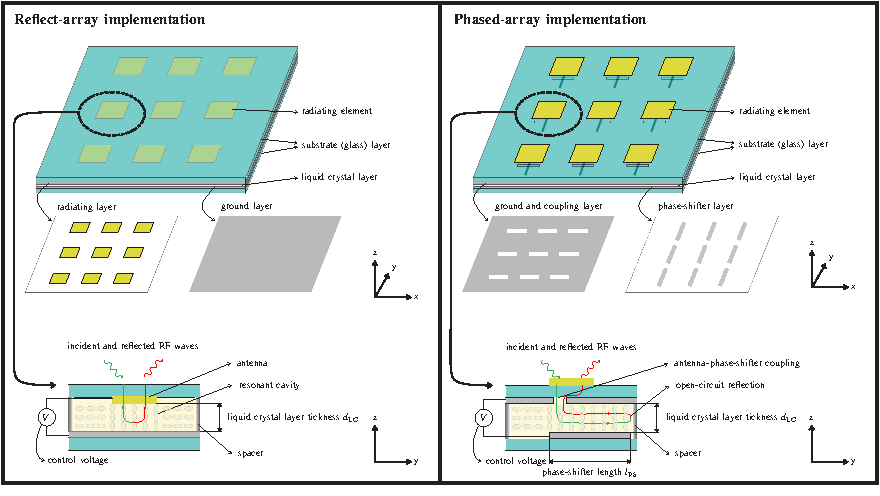
\includegraphics[width=1.9\columnwidth]{Figures/LCrisPARA.pdf}
    \caption{Schematic illustration of reflect-array vs. phased-array LC-RISs. The top figures illustrate the implementation of LC-RISs in three dimensions whereas the bottom figures show a single unit cell from $\mathsf{y}-\mathsf{z}$ cross-section. The different layers, propagation path of the RF wave, and important design parameters such as phase-shifter length $l_{\rm PS}$ (influencing the maximum phase-shift and insertion loss) and LC-layer thickness $d_{\rm LC}$ (impacting the RIS response time) are schematically illustrated.}
    \label{fig:LCrisPARA}
\end{figure*}

\textbf{Insertion loss:} The interaction of the \gls{RF} wave with the \gls{RIS} circuit introduces a certain insertion loss, $L_{\rm ins}$, which depends on the design as well as material properties such as dielectric losses, $\tan\delta$, and conductor losses. For the \gls{PA} implementation (see Section~\ref{sec:RISimplementation}), the phase-shifter length $l_{\rm PS}$ has a direct impact on the final insertion loss and maximum phase shift, see Fig.~\ref{fig:LCrisPARA}. In fact, increasing the phase-shifter length yields a higher maximum phase shift $\Delta\theta_{\max}\propto l_{\rm PS}$ at the cost of a larger insertion loss $L_{\rm ins} \propto l_{\rm PS}$. 

\textbf{Clearing point temperature:} Another physical property of \glspl{NLC} is the temperature at which an \gls{NLC} phase is converted to an isotropic liquid.  This temperature is known as the clearing point, $T_c$, after which tunability is no longer possible, and hence constitutes the highest operation temperatures. 
From the material design perspective, the main targets of \gls{NLC} design is to achieve high phase-shift contrasts, $\Delta\varepsilon $, low dielectric losses, $\tan\delta$, high clearing point temperatures, $T_c$,  and fast response times by reducing the rotational viscosity of the molecules, $\gamma_{\rm rot}$. 
The values of these parameters for several commercially available \gls{NLC} mixtures are shown in Tab.~\ref{tab:LCtypes}.

\begin{table*}
\centering
\caption{LCs for mm and sub-mm wave bands and their material properties. \cite{jakoby2020microwave}}
\label{tab:LCtypes}
\begin{tabular}{@{}lcccccccc@{}} \toprule
LC        & $\varepsilon_{r,\perp}$ & $\tan\delta_\perp$ & $\varepsilon_{r,\parallel}$ & $\tan\delta_\parallel$ & {$\Delta \varepsilon$} & $T_c (^\circ \text{C})$&  $K_{11} (\text{pN})$  &  $\gamma_{\rm rot} (\text{Pa} \cdot \text{s})$ \\ \midrule %& Ref.  &    \cite{manabe2013liquid}  &    \cite{fritzsch201977} &    \cite{weickhmann2017liquid}  &    \cite{fritzsch201977} 
K15 (5CB) & 2.7                     & 0.0273            & 3.1                         & 0.0132                & 0.4                  & 38.0            &    7.0          & 0.126                          \\
GT3-23001 & 2.41                    & 0.0141            & 3.18                        & 0.0037                & 0.77                 & 173.5           &    24           & 0.727                          \\
GT5-28004 & 2.40                    & 0.0043            & 3.32                        & 0.0014                & 0.92                 & 151.0           &    11.8         & 5.953                          \\
GT7-29001 & 2.46                    & 0.0116            & 3.53                        & 0.0064                & 1.07                 & 124.0           &    14.5         & 0.307                        \\ \bottomrule
\end{tabular}
\end{table*}

\subsection{LC-based RIS implementation} \label{sec:RISimplementation}

Next, we first discuss the basic components that are required to realize an \gls{NLC}-\gls{RIS}. Subsequently, we introduce two implementation approaches of \gls{NLC}-\glspl{RIS}, namely the \gls{RA} and \gls{PA} methods, and discuss their advantages and limitations. Both implementations are potentially compatible with current \gls{LCD} technology, which is a great advantage for the realization of cost-effective large \glspl{RIS}, see Fig.~\ref{fig:LCrisPARA}.


\textbf{Basic components:}  The thin \gls{NLC} layer is usually placed between two layers of glass. 
The choice of glass over more common materials is due to the fact that a very thin \gls{NLC} layer with a well-defined thickness needs to be achieved over large panels, therefore a stiff, smooth solid substrate is needed.
Due to its liquid state, solid spacers are needed to maintain the desired \gls{NLC} layer thickness. 
Moreover, the circuits of planar \gls{NLC} are commonly grown directly on glass substrates. Thereby, one or both sides of each glass are selectively metalized to pattern the desired circuitry, e.g., control lines and biasing electrodes. In particular, one of the glass substrates is often metalized to act as a ground layer for biasing all unit cells, whereas the other glass is selectively metalized for introducing phase-shifting control voltage of individual unit cells, see Fig. \ref{fig:LCrisPARA}. 
To receive and re-radiate the phase-shifted signal, a radiating element is needed, usually a patch or a dipole antenna. 





% Patch antenna and coupling slot
%Finally, to couple the phase shifter with free space and to be able to receive and reradiate the phase-shifted signal, a radiating element is needed. 
%This radiating element is often e.g. a patch or a dipole antenna.
%slot-coupled patch antenna so that the patch is coupled to the phase shifter on the opposite side of the ground, and the effect of tuning \gls{NLC} mainly affects the phase shifter, but not the antenna as presented in \cite{strunck2013continuously} and sketched in Fig. \ref{fig:method_PhasedArray}.

\textbf{Reflect-array implementation:} In this method, there is a common ground for all \gls{RIS} elements and the \gls{NLC} layer is directly between the antenna (acting also as one of the biasing electrodes) and the ground, see Fig. \ref{fig:LCrisPARA}. This structure forms a resonant cavity between the metal patch and the uniform ground plane. The advantage of this design is its simplicity since no patterning of the ground plane is necessary and therefore only the layer with the patches must be etched. This avoids any alignment issues during assembly. However, the limitations of this method are: \textit{i)} 
Due to the resonant effect, there is a limited bandwidth at which a nearly constant group delay and low amplitude
variations can be achieved. 
\textit{ii)} Thicker LC layers, $d_{\rm LC}$, are needed to support wideband
resonances with a low radiation quality factor to minimize
the losses. This results in slow response times, {$\tau_{\rm off}\geq 10$s}.
\textit{iii)} The LC biasing lines are comprised in the same layer of the patches and therefore need to be considered in its design.
As a guiding value, such designs achieve impedance bandwidths\footnote{The range of frequencies over which the antenna has an acceptable (-10 dB) impedance matching.} below 10\% and insertion losses in the range 6 to 10 dB.

\textbf{Phased-array implementation:} In this method, one of the glass substrates is metalized such that each \gls{RIS} element has a dedicated phase shifter (i.e., a biasing electrode). Moreover, the ground layer is patterned to couple the radiating elements to the phase-shifters, see Fig. \ref{fig:LCrisPARA}. For the realization of the phase shifters, transmission line topologies compatible with \gls{LCD} manufacturing are needed.
One of these transmission lines is the \gls{IMSL} which is depicted in Fig.~\ref{fig:LCrisPARA}. 
The transmission line should be terminated with a reflective end. % which can be achieved via an open or a short-circuit at the end of the phase shifter. For a conventional \gls{IMSL}, an \gls{RF} short circuit can be achieved by connecting the phase-sifter end to the ground, but this would also short-circuit the voltage applied for biasing. Furthermore, the realization of bias through glass compatible with mass production and very thin \gls{NLC} layers, $d_{\rm LC}< $\SI{10}{\micro\meter} remains a challenge. 
A suitable solution is the abrupt termination of the metal strip in an open end. 
Although such an open-end shows increased undesired radiation, this radiation is mainly proportional to the thickness of the \gls{NLC} layer, $d_{\rm LC}$. 
Small $d_{\rm LC} <\ $\SI{100}{\micro\meter} hence minimizes this effect.
The advantages of the \gls{PA} method are: \textit{i)} bandwidth is not limited by the phase shifter, and a thick glass in the radiating layer allows a wideband radiating element. A nearly constant group delay and low amplitude variations across the bandwidth can be achieved. 
\textit{ii)} Thin \gls{NLC} layers, $d_{\rm LC}$, are possible and lead to response times, $\tau_{\rm off}<100$~ms.
\textit{iii)} The LC biasing lines are comprised in an additional layer. They do not disturb radiation, but additional processing steps are needed to metalize and pattern the additional layer. The insertion loss of the phase shifter for thin $d_{\rm LC}$, specifically \SI{4.6}{\micro\meter}, is determined to be \SI{4.5}{\dB} for full \SI{360}{\degree} tunability at \SI{28}{\GHz} in~\cite{neuder2023compact}. The matched impedance bandwidth is expected to range around \SI{15}{\percent}. 
%Another advantage of thin layers for large surfaces is the amount of \gls{NLC} needed. Assuming \SI{100}{\micro\meter} and \SI{4.6}{\micro\meter} thicknesses for \gls{RA} and \gls{PA}, respectively, an \gls{RIS} would need $21.6$ times less \gls{NLC} for the \gls{PA} method. Even when acquiring high \gls{NLC} amounts, this difference can notably reduce the material cost. 

% Given the separation of phase shifting and the radiating layer in phased-array implementation, the thickness of glass substrate and the LC layer are indepedent. This allows to use very thin LC layers (e.g., a few µm) which reduces tuning time while having a thicker glass substrate (e.g., \ara{@AJS: can u provide a scale, a few hundred micrometer?}) which increases the bandwidth. %to  thickness in the radiating layer, which is desired to be electrically thick for large bandwidth. 
% As a result, response times as fast as tens of ms can be achieved while exhibiting large impedance bandwidth\ara{@AJS: can we say 8\%?}. The insertion loss of the phase shifter for thin $d_{\rm LC}$, specifically \SI{4.6}{\micro\meter}, is determined to be \SI{4.5}{\dB} for full \SI{360}{\degree} tunability at \SI{28}{\GHz} in~\cite{neuder2023compact}. The matched impedance bandwidth is expected to range around \SI{15}{\percent}.\vahid{Can we report impedance bandwidth and insertion loss to mirror the reflect-array method?} \alejandro{@Robin: include your achieved insertion loss values for the phase shifter, as well as expected RIS bandwidths (with radiations). 2-4 sentences to clarify difference between phase shifter and radiation element if needed.}

%A final advantage of thin layers for large surfaces is the amount of LC needed. Assuming \SI{100}{\micro\meter} and \SI{4.6}{\micro\meter} thicknesses, an \gls{RIS} would need $21.6$ times less \gls{NLC} for the phased array method. For example, $2 \times 2\ m$ \gls{RIS} would need \SI{400}{\milli \liter} and \SI{18.4}{\milli\liter}, respectively.
%Even when acquiring high \gls{NLC} amounts, this difference can notably reduce the material cost. 

%Similarly, patterning the ground plane helps improve the performance, but at the cost of an additional (3rd) selectively metalized layer.

% % Reflection - half length of phase shifter needed
% \vahid{@Alejandro: Is this paragraph valid only for phased-array implementation?} 
% \alejandro{Yes, the termination is only for phased-array implementation.}
% An important difference between the transmission-type phase shifters {\color{red} used in LCD technologies} and the reflection-type phase shifters needed for the 
%  \gls{RIS} is that the latter needs to be terminated with a reflective end. 
% This can be achieved via an open or a short-circuit at the end of the phase shifter. 
% For a conventional \gls{IMSL}, an \gls{RF} short circuit can be achieved by connecting the phase-sifter end to the ground, but this would also short-circuit the voltage applied for biasing. 
% Furthermore, the realization of bias through glass compatible with mass production and very thin \gls{NLC} layers, $d_{\rm LC}< $\SI{10}{\micro\meter} remains a challenge. 
% A viable solution is the abrupt termination of the metal strip in an open end. 
% Although such an open-end shows increased undesired radiation, this radiation is mainly proportional to the thickness of the \gls{NLC} layer, $d_{\rm LC}$. 
% Low $d_{\rm LC} <\ $\SI{100}{\micro\meter} hence minimizes this effect.  
% %Notice that a larger thickness and relative permittivity of the bottom substrate, $d_b$ and $\varepsilon_{r,b}$, also increase the radiation of the open-ended transmission line. % I am talking about the IMSL. Specify it?
% The advantage of operating the phase shifter in reflection is that the signal travels twice through it, so that the required length for a full \SI{360}{\degree} is halved compared to traditional transmission-type phase shifters for phased antenna array solutions.

% \subsection{Existing LC-based RIS experimental work}

% Recently, a few publications have shown the use of \gls{NLC} for the realization of digital metasurfaces \cite{ma2022digital}. For instance,
% \cite{wu2020liquid} presents the realization of an LC-based reflective \gls{RIS} with 1-bit programmable elements. 
% Similarly, a 1-bit design at \SI{0.645}{\tera\hertz} is presented in \cite{fu2022flexible} for transmissive RISs.  In this case, 1-bit, two-column-wise biasing is realized, so that an array of $64\times64\ $elements is controlled with 32 electrodes and the ground plane as a common electrode. The designs in \cite{wu2020liquid,fu2022flexible} follow the reflectarray implementation. In \cite{neuder2023compact}, initial works for realizing an LC-based RIS following the phased-array implementation have been reported. \alejandro{We could remove 1 or 2 references here if we have too many.}
% \ara{@AJS: I didn't get why these LC works on 1 bit and ours isn't... because in the advantages in the paragraph below we do mention continuous phase shifting as a merit}
%Differently than the design shown in Fig. \ref{fig:method_Reflectarray}, which consisted of an etched metal layer over a homogeneous ground plane, \cite{liu2021programmable} presents a \gls{NLC} metasurface which needs two patterned metallic layers to function. 
%\vahid{This reference is yet a new architecture than those in Fig.~\ref{fig:LCris} and could distract the reader. Shall we remove it? We have anyway only 15 references to cite.}
%\alejandro{Then I agree - I do not think it should be a priority.}





%Include Figure of the patch and the slot here

